%% S9: no closed S-term with a head normal form is convertible with itself applied to arguments.
%% DRAFT 2026-11-24 (skinock).  Neutral amsart shell, as S1--S8.
%% Sources: ~/Code/ski/notes/NCFP-D4.md section 11 (Theorems C and NC, with the Wizard's repairs G1, G2)
%%          and the last dated lines of ~/Code/ski/notes/A1-lock1-S3.md.
%% Paper-to-Lean map (lean-ski v1.17.0, branch ncfp-c; module Ski/NcfpC.lean, namespace Ncfp;
%% gates Ski/Audit.lean and Ski/NcfpAudit.lean):
%%   (M1) ............ Ncfp.fold_conv (Ski/Ncfp.lean; HnfS.compat, HnfS.fold_wsteps, Conv.conv_iff_join)
%%   (M2) ............ Conv.stable_iff (HnfSound.sound, HnfS.fold_hnf)
%%   (M3) ............ Ncfp.fold_apps (Ski/Ncfp.lean); Ncfp.β_ne_zero, Ncfp.fold_eq_zero
%%   lem:table (i) ... Ncfp.walkB_eq (decide +kernel; rank Ncfp.rkTable), walk_pair, β_rank, β_loop
%%   lem:table (ii) .. Ncfp.hnf12B_eq (decide +kernel), hnf12
%%   lem:walk ........ Ncfp.comb_walk; for a conversion Ncfp.thm_C, thm_C_hnf (Theorem C of the note).
%%                     Its corollaries Ncfp.cor_C, cor_C_sub, cor_C_block are subsumed by thm:main
%%                     and are not stated in the paper.
%%   thm:main ........ Ncfp.thm_NC (block form), Ncfp.thm_NC_hnf; the set Q is Ncfp.SComb, the step
%%                     p -> p' is Ncfp.scomb_closed, and S S b S^k ->> S S (b S^k) is Ncfp.comb_S_steps
%%   cor:left ........ Ncfp.ncfp_left_comb
%%   imported (A) .... Ncfp.right_combs (Ski/Ncfp.lean; S8 Theorem 2, hnf combs with teeth a_n)
%%   imported (B) .... Ncfp.cor_B1, cor_B1' (Ski/Ncfp.lean; S8 Corollary 9)
%%   imported (C) .... Ncfp.hnf2_conv (Ski/NcfpTheta.lean; S6 Lemma 4), Conv.run_hnf_hnf
%% TODO before release:
%%   1. lean-ski v1.17.0 is being released: check the tag URL in refs.bib (leanski) and add the DOI.
%%   2. S8 is in preparation: recheck the numbers "Theorem 2" and "Corollary 9" cited from it, and
%%      "Lemmas 2, 3 and 8, Theorem 9" of S1 and "Lemma 4" of S6, against the final versions.
%%   3. polonsky: no page range (LMCS vol. 16, issue 3, paper 7, published 23 July 2020; checked
%%      on Crossref and arXiv:1810.02239).  intrigila checked on Crossref.
%%   4. Wizard on this text; Grammarian on the prose.
%%   5. `make figs` regenerates fig/graph.pdf (reads fig/s1table.json).
\documentclass[11pt]{amsart}
\usepackage[T1]{fontenc}
\usepackage{lmodern}
\usepackage{amsmath,amssymb,amsthm}
\usepackage{graphicx}
\usepackage[numbers,sort]{natbib}
\usepackage[hidelinks]{hyperref}
\usepackage{bm}

\newtheorem{theorem}{Theorem}
\newtheorem{lemma}[theorem]{Lemma}
\newtheorem{corollary}[theorem]{Corollary}
\newtheorem{conjecture}[theorem]{Conjecture}

\newcommand{\Ter}{\mathcal S}
\newcommand{\red}{\twoheadrightarrow}
\newcommand{\hred}{\twoheadrightarrow_h}
\newcommand{\conv}{=_\beta}
\newcommand{\bl}{b}

\title[$S$-Terms with a Head Normal Form Absorb No Arguments]{No Closed $\bm{S}$-Term with a Head Normal Form Is Convertible with Itself Applied to Arguments}
\author{Claude Opus \& Fable with N.\ E.\ Davis}
\address{ZeroAttest, Champaign, Illinois, USA}
\email{NDavis@ZeroAttest.com}
\urladdr{https://orcid.org/0000-0002-1131-8319}
\date{\today}

\begin{document}
\begin{abstract}
We show that a closed term $p$ built from the combinator $S$ that has a head normal form is not
convertible with $p\,Y_1\cdots Y_k$, for any $k\ge1$ and closed $Y_1,\dots,Y_k$. In the 38-element
model that detects head normal forms, such a conversion is a closed walk in the graph of right
multiplication. Apart from the absorbing element $\bot$, this graph has one cycle, a loop. The loop
forces $Y_1=\dots=Y_k=S$ and a head normal form $S\,S\,p'$ with $p'$ convertible with $p'$ applied to $k$ arguments $S$.
Iterating gives an infinite comb with teeth $S$, which cannot exist. Combined with the companion
result for terms without a head normal form, the theorem shows that no closed $S$-term is
convertible with itself applied to one or more normalizing arguments. The proofs are mechanized in Lean~4.
\end{abstract}

\keywords{combinatory logic, combinator $S$, head normal form, finite model, convertibility}
\maketitle

\section{Introduction}

$\Ter$ is the set of closed terms built from $S$ by application, with $S\,x\,y\,z\to x\,z\,(y\,z)$ at
any position; $\red$ is the reflexive--transitive closure of $\to$ and $\conv$ is convertibility,
which by Church--Rosser~\citep{terese} is the existence of a common reduct. A term is
\emph{normalizing} if it reduces to a normal form, and its \emph{size} is its number of occurrences of $S$. Every $t\in\Ter$ is $S\,u_1\cdots u_m$ for a
unique $m\ge0$, with \emph{items} $u_i$; it is a \emph{head normal form} (hnf) iff $m\le2$. If
$m\ge3$, the \emph{head step} is $t\to u_1\,u_3\,(u_2\,u_3)\,u_4\cdots u_m$. Head steps give the
\emph{head run} of $t$; $\hred$ is their reflexive--transitive closure, and $t$ \emph{has an hnf} if
its head run reaches one. We write $x\,S^k$ for $x$ applied to $k$ arguments $S$.

\begin{theorem}\label{thm:main}
No $p\in\Ter$ with an hnf satisfies $p\conv p\,Y_1\cdots Y_k$ with $k\ge1$ and
$Y_1,\dots,Y_k\in\Ter$.
\end{theorem}

\begin{corollary}\label{cor:left}
No $p\in\Ter$ satisfies $p\conv p\,x_1\cdots x_k$ with $k\ge1$ and $x_1,\dots,x_k\in\Ter$
normalizing.
\end{corollary}

\noindent We import three results. In (A), $q_0,q_1,\dots$ and $a_0,a_1,\dots$ are infinite sequences in $\Ter$.
\begin{itemize}
\item[(A)] \citep[Theorem~2, for hnf combs]{s8} If $q_n\hred S\,a_n\,q_{n+1}$ for all $n$ (an infinite
  hnf comb with teeth $a_n$), then the sizes of the $a_n$ are unbounded.
\item[(B)] \citep[Corollary~9]{s8} No $p\in\Ter$ without an hnf satisfies
  $p\conv p\,x_1\cdots x_k$ with $k\ge1$ and $x_1,\dots,x_k\in\Ter$ normalizing.
\item[(C)] \citep[Lemma~4, for the model of terms modulo $\conv$]{s6} If $t\conv t'$ and the head run of $t$ reaches the hnf $S\,u_1\,u_2$,
  then the head run of $t'$ reaches an hnf $S\,u_1'\,u_2'$ with $u_1\conv u_1'$ and $u_2\conv u_2'$.
\end{itemize}
\emph{Proof of Corollary~\ref{cor:left}.} If $p$ has an hnf, Theorem~\ref{thm:main} applies; otherwise (B) applies.\qed

\section{A closed walk in the model}

Let $B=\{0,\dots,37\}$ with the table $\beta\colon B\times B\to B$ of~\citep{s1}, and $\bot=36$.
The \emph{block} of a term is $\bl(S)=0$, $\bl(f\,x)=\beta(\bl(f),\bl(x))$. We use three
facts~\citep[Lemmas~2, 3 and~8, Proposition~4, Theorem~9]{s1}.
\begin{itemize}
\item[(M1)] If $t\conv t'$, then $\bl(t)=\bl(t')$.
\item[(M2)] A term $t$ has an hnf iff $\bl(t)\ne\bot$.
\item[(M3)] $\beta(\bot,w)=\bot$ and $\beta(v,w)\ne0$ for all $v,w\in B$. Hence $\bl(t)=0$ only for $t=S$.
\end{itemize}

\begin{lemma}\label{lem:table}
\textup{(i)} There is a function $r\colon B\to\mathbb N$ such that, for all $v,w\in B$:
$\beta(v,w)=\bot$, or $r(\beta(v,w))<r(v)$, or $(v,w)=(12,0)$; and $\beta(12,0)=12$.

\textup{(ii)} For all $a,a'\in B$: $\beta(0,a)\ne12$, and $\beta(\beta(0,a),a')=12$ only if $a=0$.
\end{lemma}

\begin{proof}
Each statement is checked on all $38^2$ cases of the table, with $r$ as in Figure~\ref{fig:graph}.
\end{proof}

\begin{figure}[t]
\centering
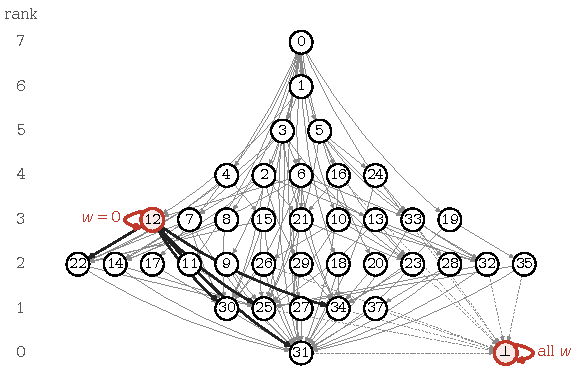
\includegraphics[width=0.9\textwidth]{fig/graph.pdf}
\caption{The graph of right multiplication on the 38 blocks: an arrow $v\to u$ means
$u=\beta(v,w)$ for some $w$. Each block other than $\bot$ is in the row of its rank $r$, the
length of the longest walk from it that avoids $\bot$ and the loop at $12$; $r(\bot)=0$. All 107
arrows between distinct blocks other than $\bot$ lead to a lower row; those from $12$ are drawn
black, the others grey. Eleven blocks have an arrow to $\bot$ (dashed). The only cycles are the
loops at $\bot$ and at $12$: $\beta(\bot,w)=\bot$ for every $w$, and $\beta(12,w)=12$ only for
$w=0$.}
\label{fig:graph}
\end{figure}

\begin{lemma}\label{lem:walk}
Let $p,Y_1,\dots,Y_k\in\Ter$ with $k\ge1$. If $\bl(p\,Y_1\cdots Y_k)=\bl(p)\ne\bot$, then
$Y_1=\dots=Y_k=S$ and $\bl(p)=12$.
\end{lemma}

\begin{proof}
Let $v_i=\bl(p\,Y_1\cdots Y_i)$, so that $v_i=\beta(v_{i-1},\bl(Y_i))$ and $v_k=v_0\ne\bot$. No
$v_i$ is $\bot$: otherwise (M3) gives $v_k=\bot$. By Lemma~\ref{lem:table}(i), $r(v_i)\le r(v_{i-1})$ for $1\le i\le k$, with
equality only if $v_{i-1}=v_i=12$ and $\bl(Y_i)=0$. Since $r(v_k)=r(v_0)$, equality holds for
every $i$. So $v_0=12$, and every $Y_i$ is $S$ by (M3).
\end{proof}

\section{Proof of Theorem~\ref{thm:main}}

Let $Q$ be the set of $p\in\Ter$ that have an hnf and satisfy $p\conv p\,Y_1\cdots Y_k$ for some
$k\ge1$ and $Y_1,\dots,Y_k\in\Ter$. We show that every $p\in Q$ satisfies $p\hred S\,S\,p'$ for
some $p'\in Q$. Then, if $Q$ had an element $q_0$, it would start a sequence with
$q_n\hred S\,S\,q_{n+1}$ for all $n$. The teeth $S$ have size $1$, so the sizes are bounded,
against (A).

Let $p\in Q$. By (M1) and (M2), $\bl(p\,Y_1\cdots Y_k)=\bl(p)\ne\bot$, so by Lemma~\ref{lem:walk}
all $Y_i$ are $S$ and $\bl(p)=12$. Let $h$ be the hnf on the head run of $p$; then $\bl(h)=12$
by (M1). Now $h\ne S$, since $\bl(S)=0$, and $h\ne S\,a$ by Lemma~\ref{lem:table}(ii). So
$h=S\,a\,p'$ with $\beta(\beta(0,\bl(a)),\bl(p'))=12$. Hence $\bl(a)=0$ by
Lemma~\ref{lem:table}(ii), and $a=S$ by (M3). So $p\hred S\,S\,p'$.

Each term on the head run of $p$ before $h$ has at least three items, so the head run of
$p\,S^k$ copies it, with $S^k$ appended, and reaches $S\,S\,p'\,S^k$. Each of the next $k$ head
steps is $S\,S\,x\,S\to S\,S\,(x\,S)$, with the remaining arguments appended. So
$p\,S^k\hred S\,S\,(p'\,S^k)$, which is an hnf. Since $p\conv p\,S^k$, (C) applied to $p\,S^k$ and $p$ gives an hnf
$S\,u_1\,u_2$ on the head run of $p$ with $u_2\conv p'\,S^k$. The head run is deterministic and
stops at its first hnf, so $S\,u_1\,u_2=h=S\,S\,p'$, and $p'\conv p'\,S^k$. As $S$ is normal, (B)
then gives $p'$ an hnf. So $p'\in Q$.\qed

\section{Closing}

Lemma~\ref{lem:walk} does not give the theorem alone: the terms $q=S\,S\,(S\,(S\,S))$ and
$q\,S$ both have block $12$. For $p$ without an hnf the walk stays at $\bot$ and says nothing.
There, by~(B), a solution needs some $Y_i$ without a normal form.

\begin{conjecture}
No $p,Y_1,\dots,Y_k\in\Ter$ with $k\ge1$ satisfy $p\conv p\,Y_1\cdots Y_k$.
\end{conjecture}

\noindent In the $\lambda$-calculus every equation $p\conv p\,x$ has a solution, by the fixed-point
theorem. Statman conjectured that no fixed-point combinator $Y$ satisfies $Y\conv Y\,\delta$, where
$\delta=\lambda yx.\,x\,(y\,x)$. Intrigila~\citep{intrigila} published a proof; Polonsky~\citep{polonsky}
still states the claim as a conjecture. For $S$ alone, Corollary~\ref{cor:left} shows that
$p\conv p\,x$ has no solution with $x$ normalizing.

\section*{Data availability}
\sloppy
Every result of this paper is proved in the Lean~4~\citep{lean4} development
\texttt{lean-ski}~\citep{leanski}, version 1.17.0: Theorem~\ref{thm:main}, its corollary and the
lemmas in module \texttt{Ski/NcfpC.lean}, (A) and~(B) in \texttt{Ski/Ncfp.lean}, and (C) in
\texttt{Ski/NcfpTheta.lean} and \texttt{Ski/Conv.lean}; (M1)--(M3) are \texttt{Ncfp.fold\_conv},
\texttt{Conv.stable\_iff} and \texttt{Ncfp.fold\_eq\_zero}. The proofs use only the axioms
\texttt{propext} and \texttt{Quot.sound}.
Lemma~\ref{lem:table} is checked in the Lean kernel by \texttt{decide +kernel}. The Lean proof of
Theorem~\ref{thm:main} uses (A) in its form for a set of terms closed under $p\mapsto p'$, so it
chooses no sequence. The script \texttt{fig/graph.py} draws the figure and recomputes $r$ from the
table of~\citep{s1}.

\bibliographystyle{plainnat}
\bibliography{refs}
\end{document}
